\documentclass[a4paper,12pt]{article}
\usepackage[utf8]{inputenc}
\usepackage{graphicx}
\usepackage{listings}
\usepackage{listingsutf8}
\usepackage{url}
\usepackage{amsmath}
%\title{TFG}
%\author{Miguel Ardura Zorita}
%\date{}
\usepackage{color}

\definecolor{mygreen}{rgb}{0,0.6,0}
\definecolor{mygray}{rgb}{0.5,0.5,0.5}
\definecolor{mymauve}{rgb}{0.58,0,0.82}

\lstset{ %
  backgroundcolor=\color{white},   % choose the background color; you must add \usepackage{color} or \usepackage{xcolor}
  basicstyle=\footnotesize,        % the size of the fonts that are used for the code
  breakatwhitespace=false,         % sets if automatic breaks should only happen at whitespace
  breaklines=true,                 % sets automatic line breaking
  captionpos=b,                    % sets the caption-position to bottom
  commentstyle=\color{mygreen},    % comment style
  deletekeywords={...},            % if you want to delete keywords from the given language
  escapeinside={\%*}{*)},          % if you want to add LaTeX within your code
  extendedchars=true,              % lets you use non-ASCII characters; for 8-bits encodings only, does not work with UTF-8
  frame=single,	                   % adds a frame around the code
  keepspaces=true,                 % keeps spaces in text, useful for keeping indentation of code (possibly needs columns=flexible)
  keywordstyle=\color{blue},       % keyword style
  language=Octave,                 % the language of the code
  otherkeywords={*,...},           % if you want to add more keywords to the set
  numbers=left,                    % where to put the line-numbers; possible values are (none, left, right)
  numbersep=5pt,                   % how far the line-numbers are from the code
  numberstyle=\tiny\color{mygray}, % the style that is used for the line-numbers
  rulecolor=\color{black},         % if not set, the frame-color may be changed on line-breaks within not-black text (e.g. comments (green here))
  showspaces=false,                % show spaces everywhere adding particular underscores; it overrides 'showstringspaces'
  showstringspaces=false,          % underline spaces within strings only
  showtabs=false,                  % show tabs within strings adding particular underscores
  stepnumber=2,                    % the step between two line-numbers. If it's 1, each line will be numbered
  stringstyle=\color{mymauve},     % string literal style
  tabsize=2,	                   % sets default tabsize to 2 spaces
  title=\lstname                   % show the filename of files included with \lstinputlisting; also try caption instead of title
}
\begin{document}
\lstset{inputencoding=utf8/latin1}
\renewcommand{\figurename}{Figura}
\begin{titlepage}
\begin{center}
\begin{figure}
\begin{center}

\includegraphics[width=8cm]{logo.jpg}
\end{center}
\end{figure}
FACULTAD DE MATEMÁTICAS\\
\vspace{0.2in}
\begin{Large}
\textbf{Técnicas de preprocesado y procesado de imágenes astronómicas mediante OpenCV}
\end{Large}
\rule{80mm}{0.1mm}\\
%\maketitle
\begin{large}
Miguel Ardura Zorita\\
Director: Carlos Gregorio Rodríguez
\end{large}
\vspace*{0.3in}
\rule{80mm}{0.1mm}\\
\vspace*{0.1in}

\end{center}

\end{titlepage}

\newpage
\section*{Abstract}
Here goes the English version of the abstract.
\\
\newpage
\renewcommand\contentsname{Índice general}
\tableofcontents
\newpage
\section{Motivación}
Este trabajo tenía la tarea radical de servirme de una primera aproximación a la disciplina de la Visión Artificial. Si bien aquí se presenta una aplicación concreta al campo de la Astronomía, mi objetivo era conocer las técnicas utilizadas en la creación, manipulación y procesado de imágenes mediante las herramientas de que se dispone ahora, tanto de hardware como de software. La elección concreta de la Astronomía como campo de estudio surgió al poco de reunirme con mi tutor, Carlos Gregorio, y responde a mi afición por tal ciencia y deseo de poder experimentar con las imágenes generadas por los telescopios a un nivel superior al de un mero aficionado.
\\
Aunque en el camino se ha ido variando el rumbo del proyecto en multitud de ocasiones, finalmente decidí centrarlo en la detección semi-automática de galaxias tomando como input un fichero FITS\footnote{Ver la sección \ref{sec:FITS}} para una posterior clasificación en un trabajo futuro. El resultado del procesado es la detección de las estructuras candidatas a galaxias a través de sus contornos y la identificación de los objetos más brillantes de la imagen, con el fin de simplificar un trabajo posterior de discriminización de objetos no candidatos a galaxias.


\section{Herramientas usadas}

En esta sección se informa brevemente de las herramientas que he utilizado a lo largo del proyecto, tanto los tipos de ficheros (FITS), como las librerías usadas (Astropy, OpenCV, Numpy, Matplotlib).
\subsection{Ficheros FITS}
\label{sec:FITS}

FITS son las siglas de Flexible Image Transport System, un formato de archivo que sirve para recoger, transportar y procesar datos consistentes en arrays multidimensionales y tablas que almacenan información con la estructura clave-valor, siendo éstos principalmente imágenes científicas y metadatos.
\subsubsection{Astropy}
\subsection{OpenCV}
\subsubsection{Kernel en imágenes}
\label{sec:Kernel}
\subsection{Numpy}
\subsection{Matplotlib}
\section{Desarrollo del proyecto}
\subsection{Procesado de los ficheros FITS}

El proceso de tratado de las imágenes empieza con la carga y lectura de los ficheros FITS. Esto se hace por medio de la librería Astropy. Como se explica en la sección \ref{sec:FITS}, la matriz que representa la imagen que se usará aquí se corresponde con el primer HDU. Así, el siguiente código carga en 'img' el ndarray de numpy contenido en el archivo FITS de muestra:

\lstinputlisting[language=Python, frame= single, firstline=1, lastline=5]{basicLoading.py}

El siguiente código hace uso de OpenCV para mostrar la imagen antes cargada. Se realiza un mapeo lineal de los valores leídos del FITS a [0,1] para normalizar los valores de la imagen y que la función \textbf{imshow} no aparezca en blanco debido a la conversión al rango [0,255] que \textbf{imshow}\footnote{\url{http://docs.opencv.org/2.4/modules/highgui/doc/user_interface.html#imshow}} realiza a las imágenes en float 32:

\lstinputlisting[language=Python, frame= single, firstline=7]{basicLoading.py}

La figura \ref{fig:img1} muestra la imagen cargada con el script anterior.
\begin{figure}[h!]
\centering
\fbox{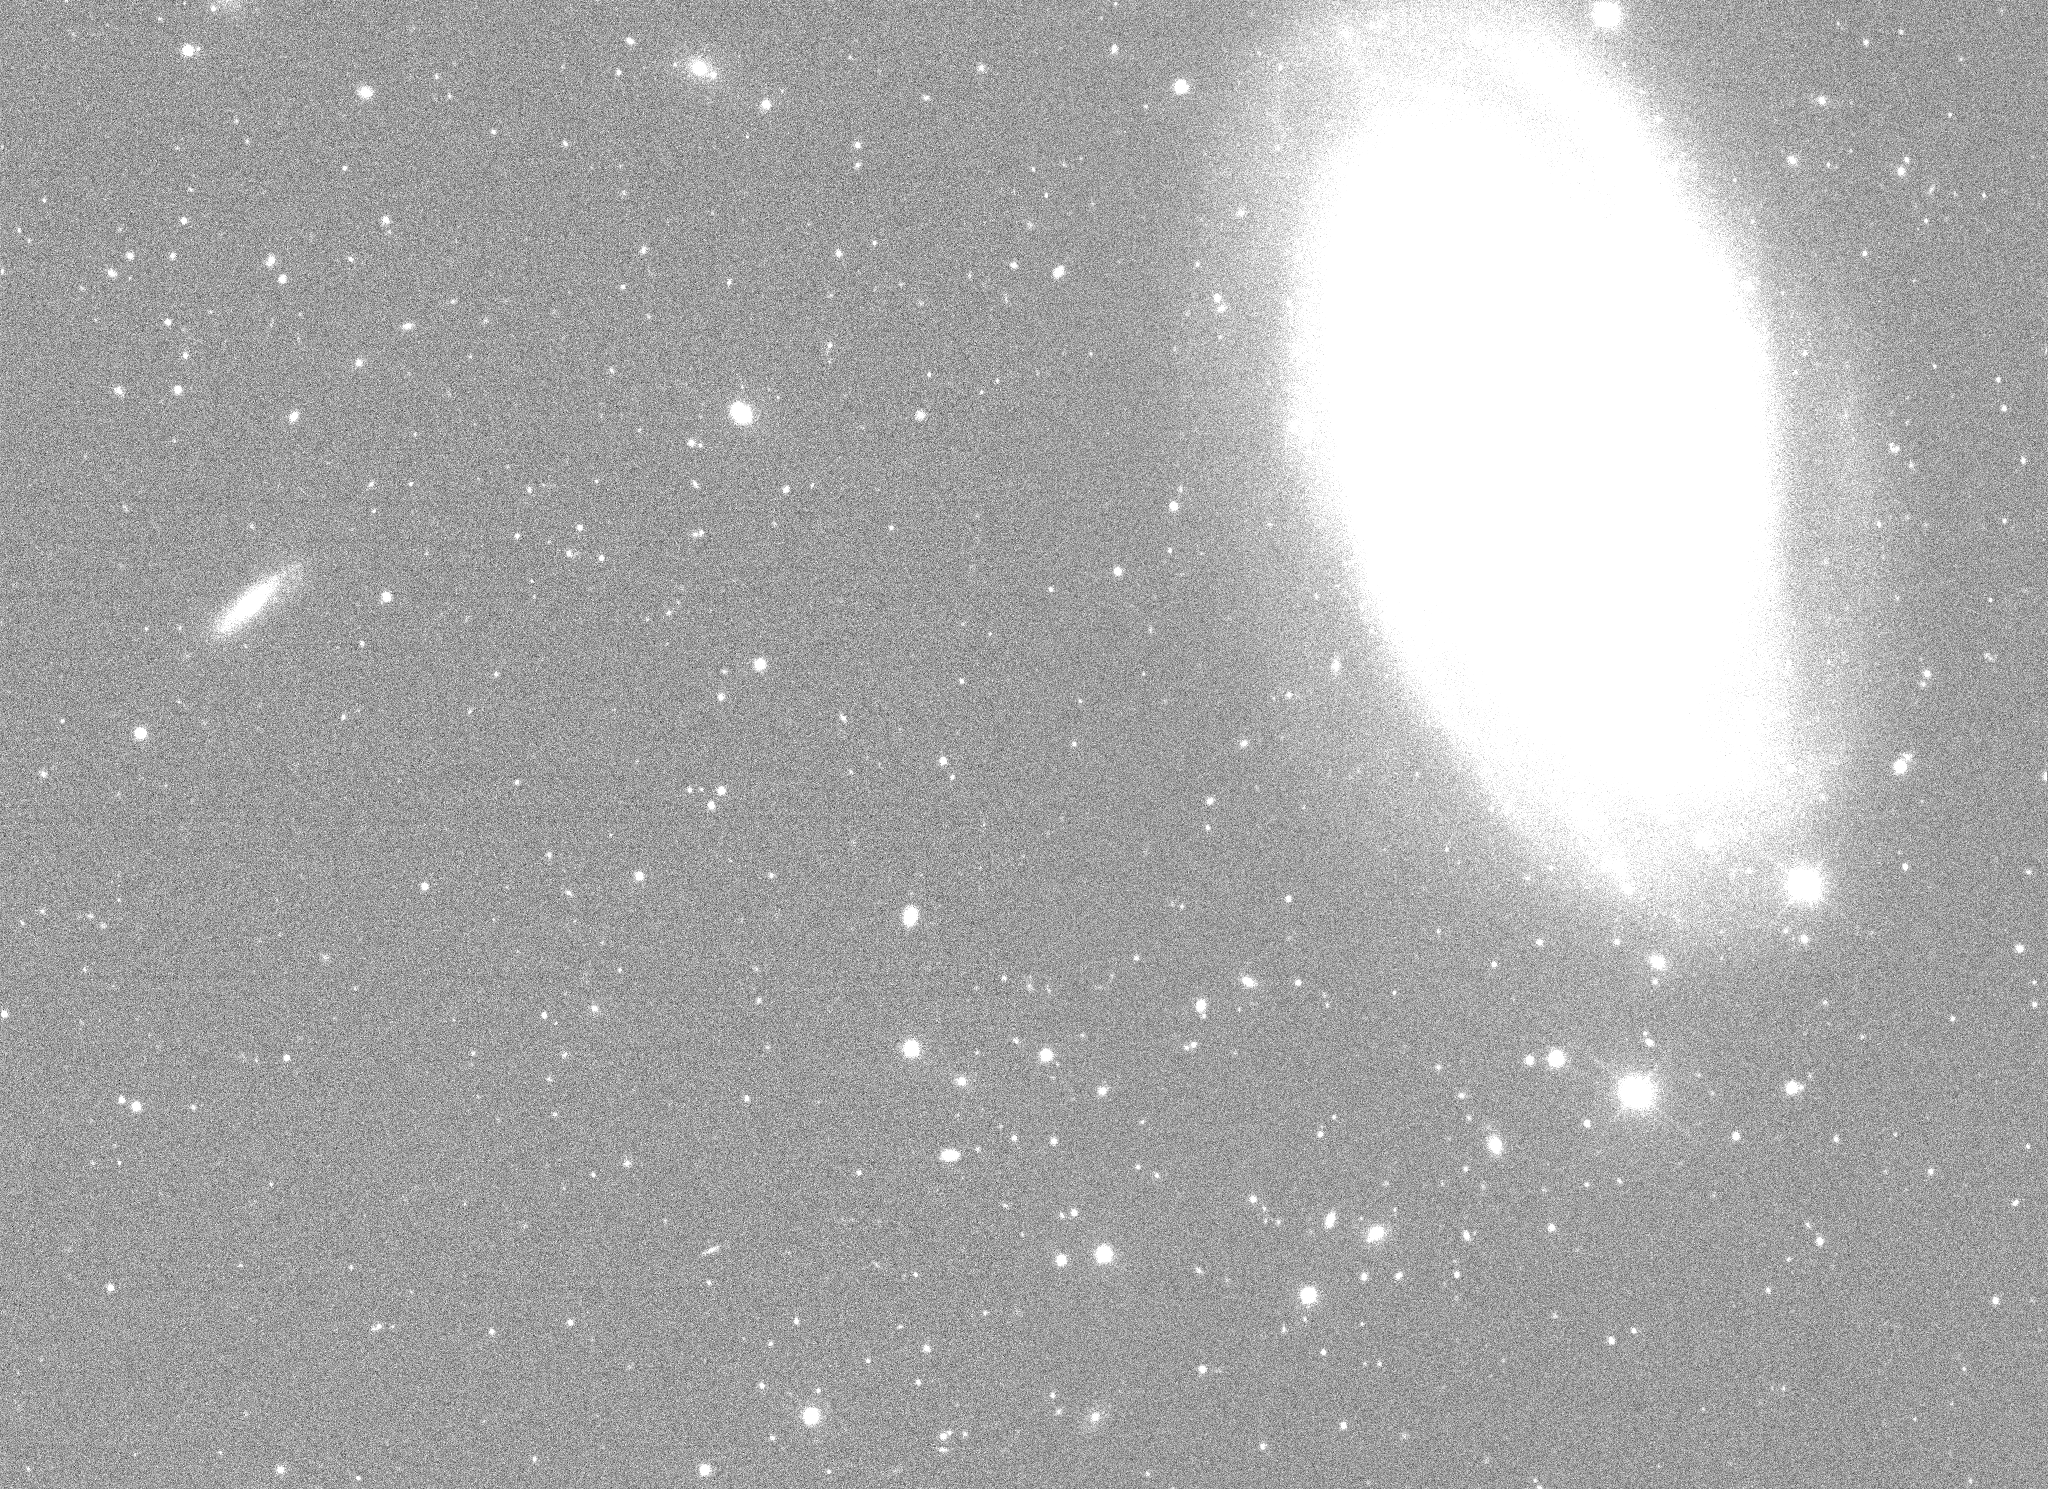
\includegraphics[width=10cm]{img1.png}}
\caption{Visualización del archivo frame-i-002830-6-0398.fits por medio de \textit{basicLoading.py}.}
\label{fig:img1}
\end{figure}

\subsection{Uso de un filtro customizado}

Ante la problemática surgida en lo que respecta a la eliminación del ruido de las imágenes haciendo uso de las herramientas predefinidas en la librería OpenCV (como se muestra en la sección \ref{sec:Problemas}), creé un filtro con el que obtengo resultados más cercanos a lo que quería. En concreto consiste en el uso del método \textbf{filter2D}\footnote{\url{http://docs.opencv.org/2.4/modules/imgproc/doc/filtering.html#filter2d}} de OpenCV. Dicho método sirve para crear un filtro a partir de un kernel (véase la sección \ref{sec:Kernel}) dado.
En concreto, creé el kernel
$\begin{pmatrix}
0 & 1 & 0 \\
1 & 0 & 1 \\
0 & 1 & 0
\end{pmatrix}$
y lo usé en la primera etapa del procesado de las imágenes.
Tomando la imagen resultado de aplicar este filtro a la imagen leída de los archivos FITS, y aplicando técnicas de segmentación, obtuve resultados con los que pude seguir avanzando.

\subsection{Segmentación}

Me encontré con que, junto con la aplicación del filtro que creé, las técnicas de segmentación de las que provee OpenCV eran suficiente para eliminar gran cantidad del ruido existente en las imágenes. Esto me es de gran utilidad en el proceso de la detección de galaxias porque reduce enormemente la cantidad de información no útil para este propósito, como las regiones vacías o en las que los objetos luminosos no aparecen agrupados de forma ordenada.

En concreto uso el método de \textit{thresholding}, que es una técnica de segmentación que consiste en una identificación de los valores de la imagen a través de una relación de equivalencia dada. En términos de Teoría de Conjuntos esto equivale a la construcción del espacio cociente del conjunto de píxeles por medio de la relación de equivalencia que dicte el método, y en el que a los píxeles relacionados se les asignará el mismo valor en el espacio cociente resultante.

Tales relaciones son, en el caso de segmentación por \textit{thresholding}, de comparación con un umbral dado. OpenCV ofrece cinco tipos de segmentación usando este método\footnote{\url{http://docs.opencv.org/2.4/modules/imgproc/doc/miscellaneous_transformations.html?highlight=threshold#threshold}}. A saber:

\begin{itemize}
\item \textbf{Binario:} Fijado un umbral, si el valor de un píxel excede ese umbral, se le asigna un valor fijado como máximo; si no, se le asignará 0.
\item \textbf{Binario invertido:} Análogo al anterior, pero con las condiciones invertidas.
\item \textbf{Truncado:} Si el valor de un píxel excede el umbral, se le asignará el umbral como nuevo valor. En caso contrario no se ve alterado.
\item \textbf{Truncado a cero:} Si el valor de un píxel es menor que el del umbral, se le asigna el valor cero. En caso contrario no se ve alterado.
\item \textbf{Truncado a cero invertido:} Análogo al anterior, pero con las condiciones invertidas.
\end{itemize}

El que me daba mejores resultados y decidí usar es el binario invertido.

En lo que respecta a los parámetros de la función, encontré que el umbral obtenido automáticamente por el algoritmo de Otsu y el valor máximo igual a 1 daban los resultados más aproximados a lo que buscaba.
El siguiente código recoge la aplicación de esto anterior:
\lstinputlisting[language=Python, frame= single]{customFilter+thresholding.py}
y la figura \ref{fig:img2} muestra la imagen que es generada por el código anterior a partir de la imagen antes vista.

\begin{figure}[h!]
\centering
\fbox{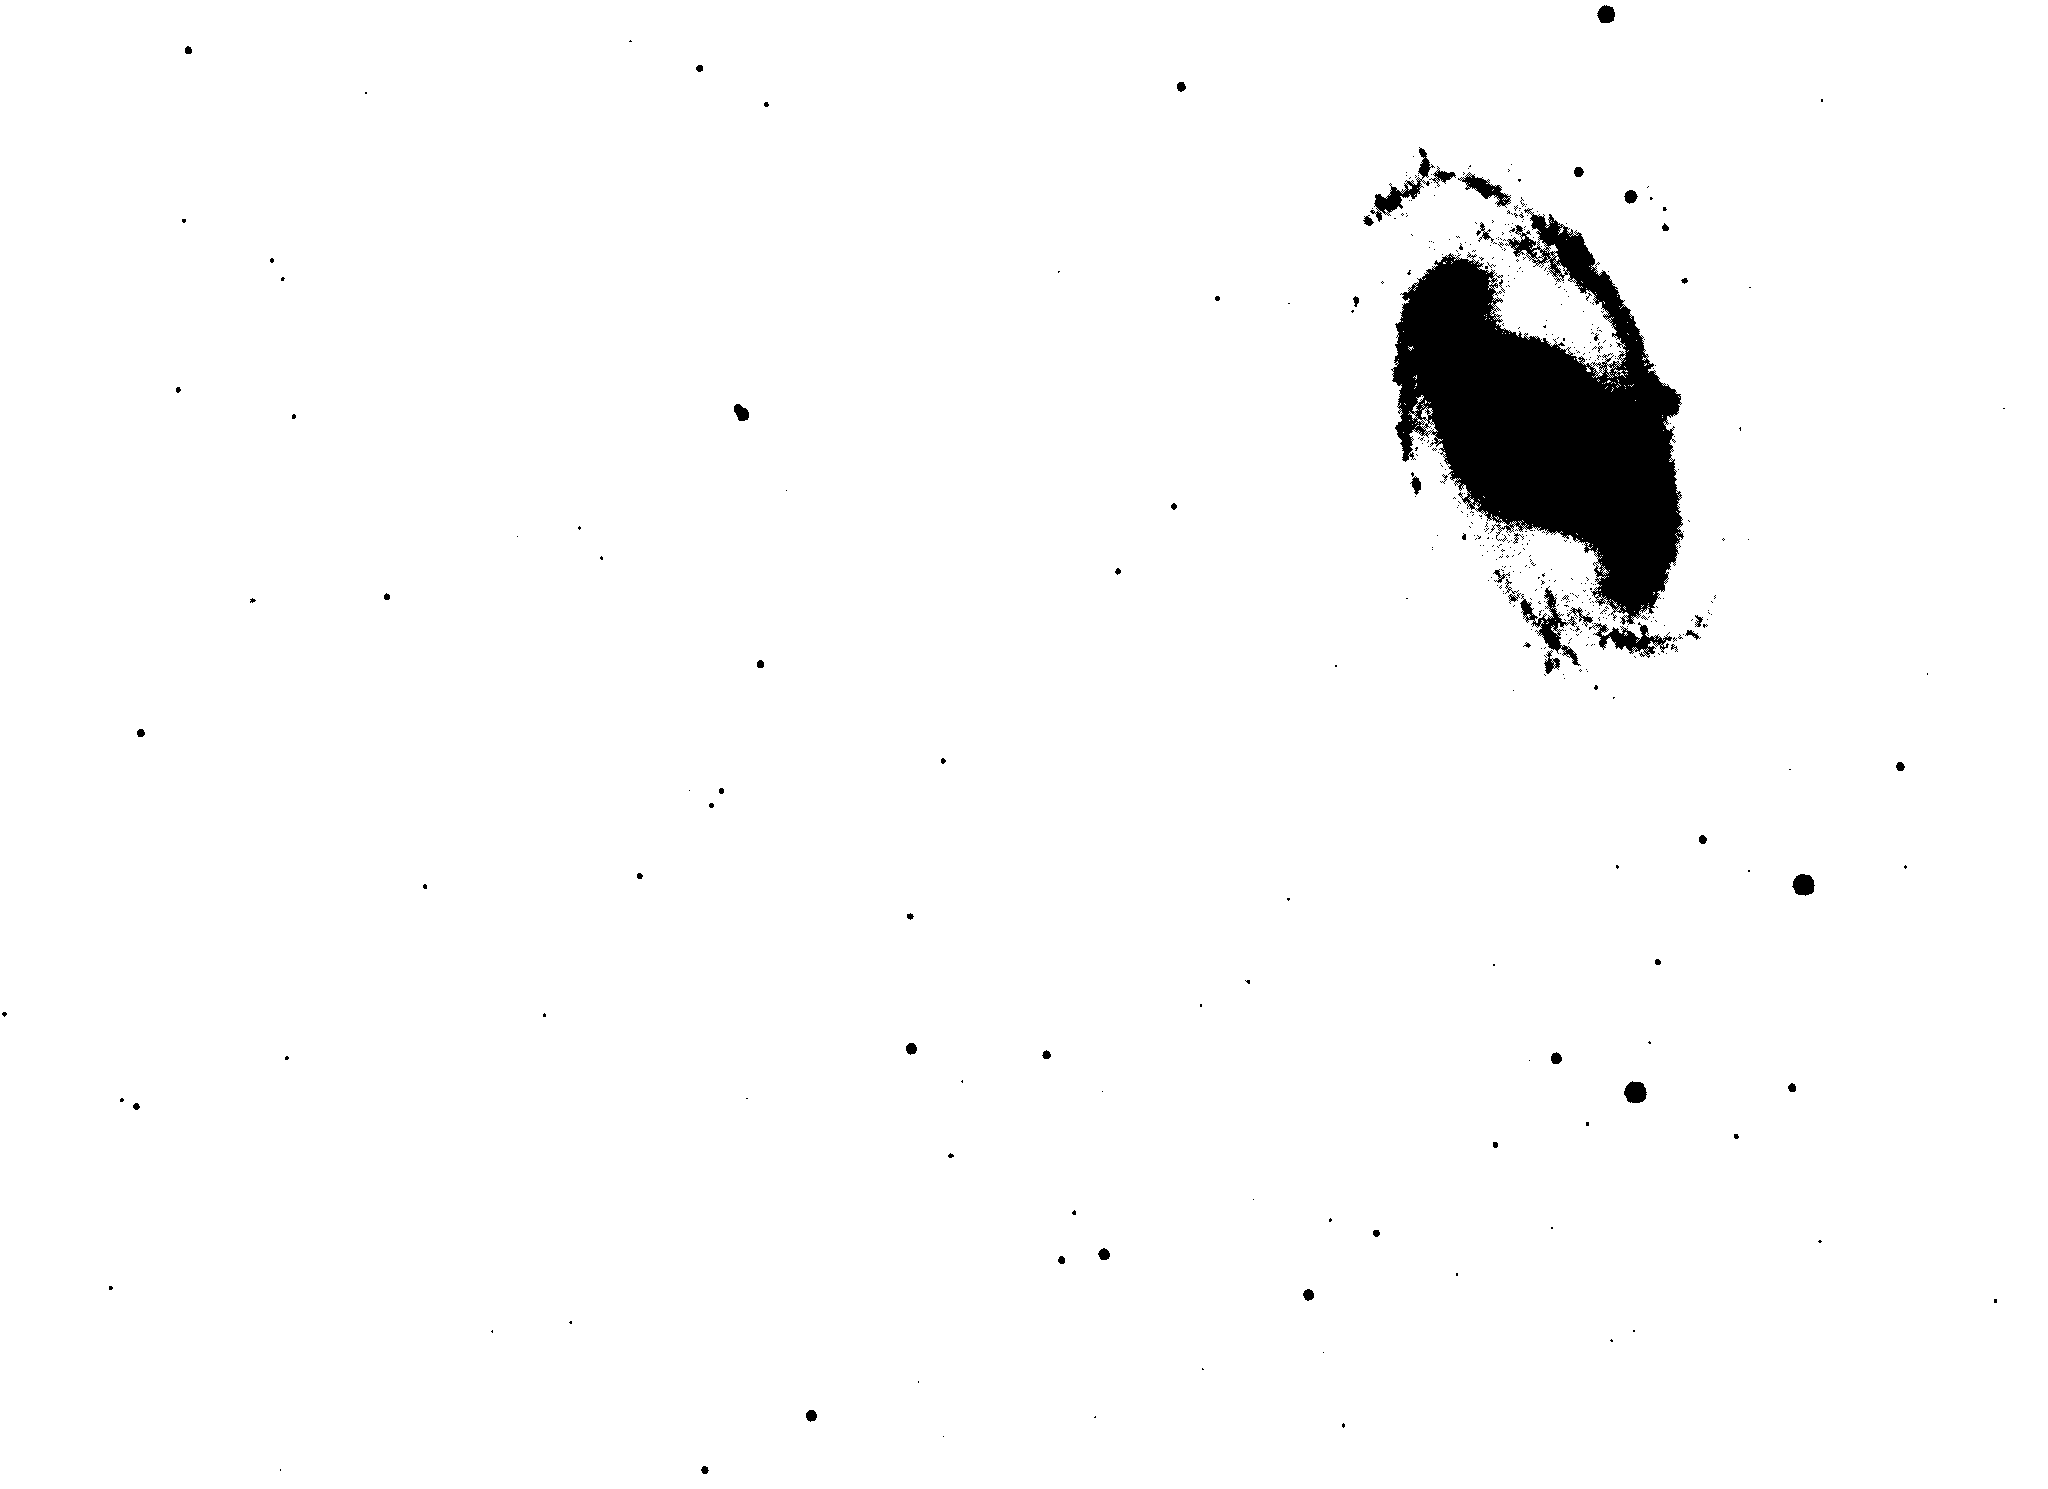
\includegraphics[width=8cm]{img2.png}}
\caption{Imagen resultado de aplicar lo anterior a la imagen vista antes.}
\label{fig:img2}
\end{figure}

Como se puede observar, gran parte del granulado de la imagen original ha desaparecido y en su lugar se distinguen motas aisladas y una gran estructura. Se aprecia claramente una zona central de la que salen brazos finos hacia el exterior.

A fin de conseguir que esta detección fuera automática, introduje el estudio de \textit{contornos} en la imágenes obtenidas, lo que lleva a la siguiente etapa del procesado.

\subsection{Detección de contornos}
Con el fin de identificar y aislar las regiones oscuras que aparecen aplicando \textit{thresholding}, incorporo el uso del método que detecta contornos \textbf{findContours}\footnote{\url{http://docs.opencv.org/2.4/modules/imgproc/doc/structural_analysis_and_shape_descriptors.html?highlight=findcontours#findcontours}} de OpenCV. Este método toma como input una imagen de 8 bits, un modo y un método y devuelve la lista de contornos. Como modo utilizo el que devuelve los contornos en una estructura anidada (\textbf{RETR\_TREE}), y como método de aproximación de los contornos, uso el que comprime los segmentos para almacenar solo sus extremos (\textbf{CHAIN\_APPROX\_SIMPLE}). El objetivo es usar el método de OpenCV que determina el rectángulo que se ajusta a cada contorno, y entre todos esos rectángulos quedarse con el de mayor área, que es el que contiene al contorno candidato a estructura de interés. Para esto hago uso del método \textbf{boundingRect}\footnote{\url{http://docs.opencv.org/2.4/modules/imgproc/doc/structural_analysis_and_shape_descriptors.html?highlight=findcontours#boundingrect}}, que dado un contorno, devuelve cuatro parámetros que corresponden a las dos coordenadas del vértice superior izquierdo, la base y la altura del rectángulo horizontal que ajusta al contorno.


El siguiente script muestra su uso:
\lstinputlisting[language=Python, frame= single]{contours+BoundingRects.py}
y la figura \ref{fig:img3} muestra la imagen resultante.

\begin{figure}[h!]
\centering
\fbox{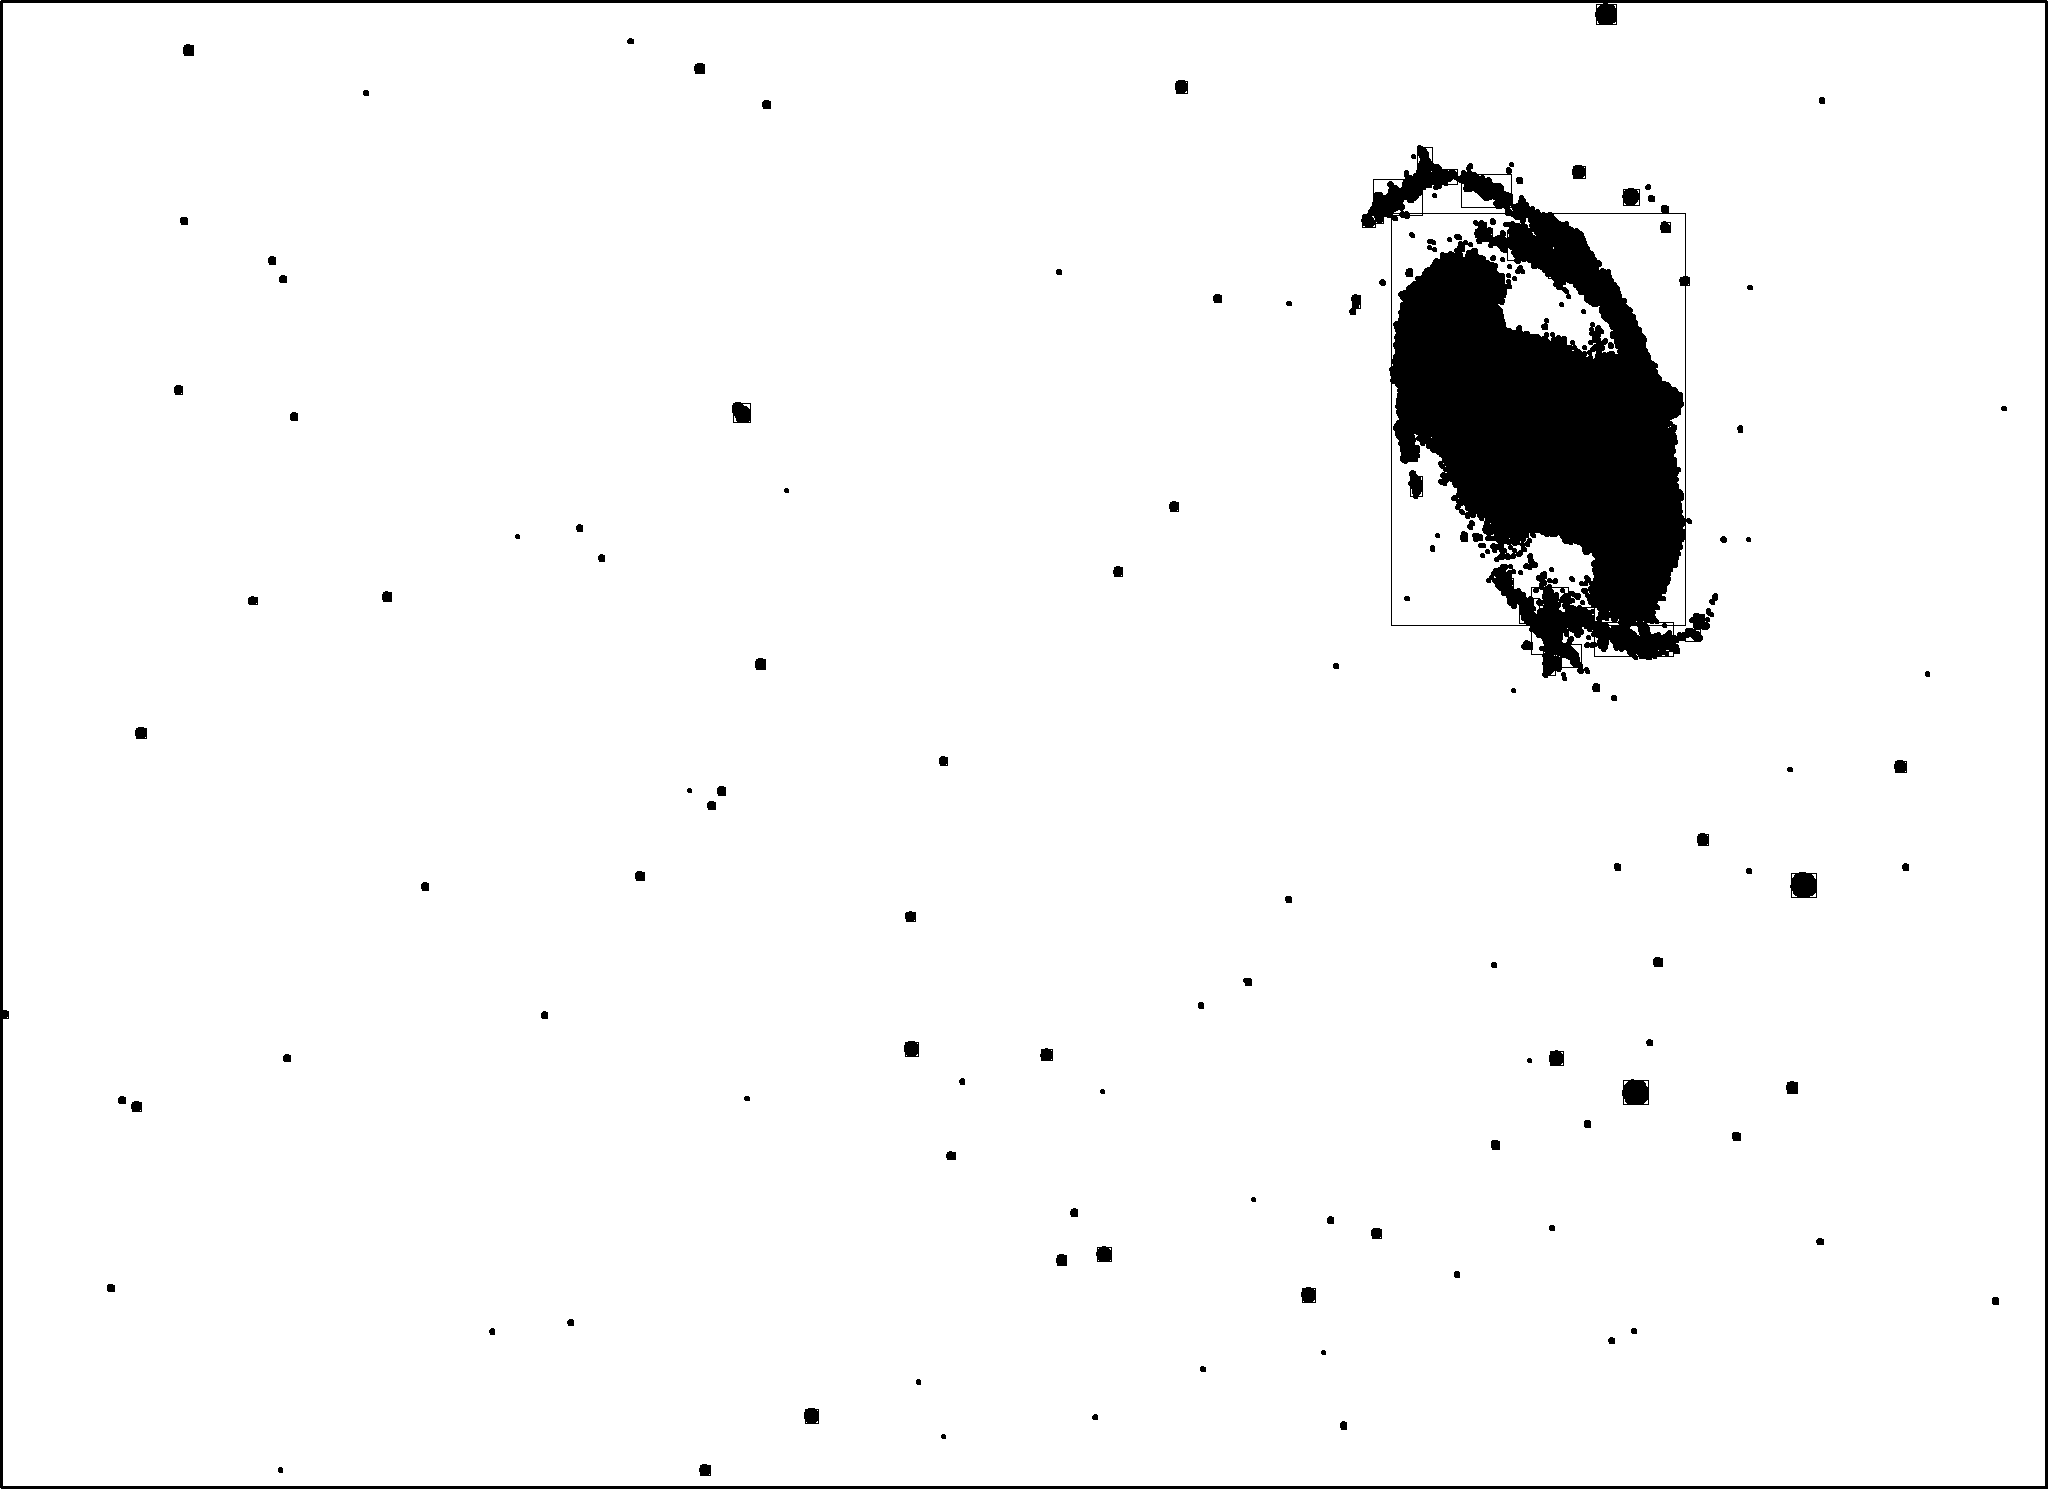
\includegraphics[width=8cm]{img3.png}}
\caption{Rectángulos ajustando los contornos.}
\label{fig:img3}
\end{figure}
Para determinar el rectángulo de mayor área, se predefine un rectángulo inicial de alto y ancho iguales a cero para en cada iteración sobre los contornos comparar el rectángulo que ajusta al contorno de la iteración con el de máximo área actual. Se corresponde con la siguiente sección del código:
\lstinputlisting[language=Python, frame= single, firstline=25, lastline=29]{contours+BoundingRects.py}
La condición $w*h<2040*1480$ descarta el contorno que corresponde al borde exterior de la imagen, pues eventualmente puede aparecer como resultado del cálculo de contornos.

La figura \ref{fig:img3Rect} muestra el resultado de recortar la imagen \ref{fig:img3} por el rectángulo de mayor área detectado.

\begin{figure}[h!]
\centering
\fbox{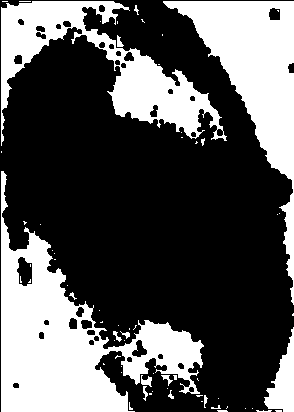
\includegraphics[width=4cm]{img3Rect.png}}
\caption{Recorte del contorno identificado.}
\label{fig:img3Rect}
\end{figure}



\subsection{Estudio en paralelo: detección de candidatos a estrellas}
Con el fin de identificar todas las posibles galaxias presentes en la imagen, surge la necesidad de determinar cuándo una región luminosa se corresponde con una estrella y cuándo con una galaxia, pues ambos objetos pueden presentar tamaños y formas similares.

A diferencia de la discretización anterior, me centro ahora en la identificación de los objetos que por su luminosidad se destacan sobre su alrededor. Para ello hago un uso combinado del filtro customizado y función de \textit{thresholding} antes mencionados, y lo combino con la función \textbf{morphology}\footnote{\url{http://docs.opencv.org/2.4/modules/imgproc/doc/filtering.html?highlight=morphologyex#morphologyex}} de OpenCV, que proporciona herramientas para el uso de transformaciones morfológicas.

Una transformación morfológica es básicamente una operación que provee de información sobre la estructura de una imagen por medio de la aplicación de un elemento estructurador. Generalmente consistirá en la convolución de la imagen de partida con un kernel. La naturaleza de este kernel será lo que determine la imagen resultado.

Las transformaciones implementadas disponibles en \textbf{morphology} se basan en dos operaciones básicas: la \textit{dilatación} y la \textit{erosión}. En ambos casos se convoluciona con un kernel que generalmente tiene forma rectangular o circular y a cada píxel se le asigna un nuevo valor dependiendo de los valores de los píxeles que lo rodeen . En el caso de la dilatación se toma el máximo valor de los píxeles del entorno definido por el kernel, y en el caso de la erosión el mínimo. Cuando la imagen es binaria estos valores se corresponden con 1 y 0 respectivamente.

Combinando estas dos transformaciones, OpenCV dispone de las siguientes operaciones:
\begin{itemize}
\item \textbf{Apertura (open): } es el resultado de aplicar una erosión seguida de una dilatación.
\begin{center}
$apertura(imagen, kernel) = dilataci\acute{o}n(erosi\acute{o}n(imagen,kernel), kernel)$
\end{center}
\item \textbf{Cierre (close):} es el resultado de aplicar una dilatación seguida de una erosión.
\begin{center}
$cierre(img, kernel) = erosi\acute{o}n(dilataci\acute{o}n(imagen,kernel),kernel)$
\end{center}
\item \textbf{Gradiente:} es la diferencia de la erosión y la dilatación de una imagen.
\begin{center}
$gradiente(imagen, kernel) = dilataci\acute{o}n(imagen,kernel) - erosi\acute{o}n(imagen,kernel)$
\end{center}
\item \textbf{Top Hat:} es la diferencia de la imagen inicial y su apertura.
\begin{center}
$tophat(imagen, kernel) = imagen - apertura(imagen, kernel)$
\end{center}
\item \textbf{Black Hat:} es la diferencia del cierre y la imagen inicial.
\begin{center}
$blackhat(imagen, kernel) = cierre(imagen, kernel)- imagen$
\end{center}
\end{itemize}

Se puede ver un ejemplo de la aplicación de estas operaciones en la sección \ref{sec:morf}.

A través de la experimentación encontré que la operación cierre conseguía descartar la mayor cantidad de ruido de la mayoría de las imágenes, salvo en algunos casos, en los que por la naturaleza de las imágenes los procedimientos aquí usados dan resultados erróneos (véase sección \ref{sec:Problemas}.

El siguiente código muestra el uso de la operación cierre:
\lstinputlisting[language=Python, frame= single, firstline=1, lastline=16]{blobDetection.py}
y la figura \ref{fig:img4} muestra la imagen resultante de aplicar en cinco iteraciones la operación cierre.
\begin{figure}[h!]
\centering
\fbox{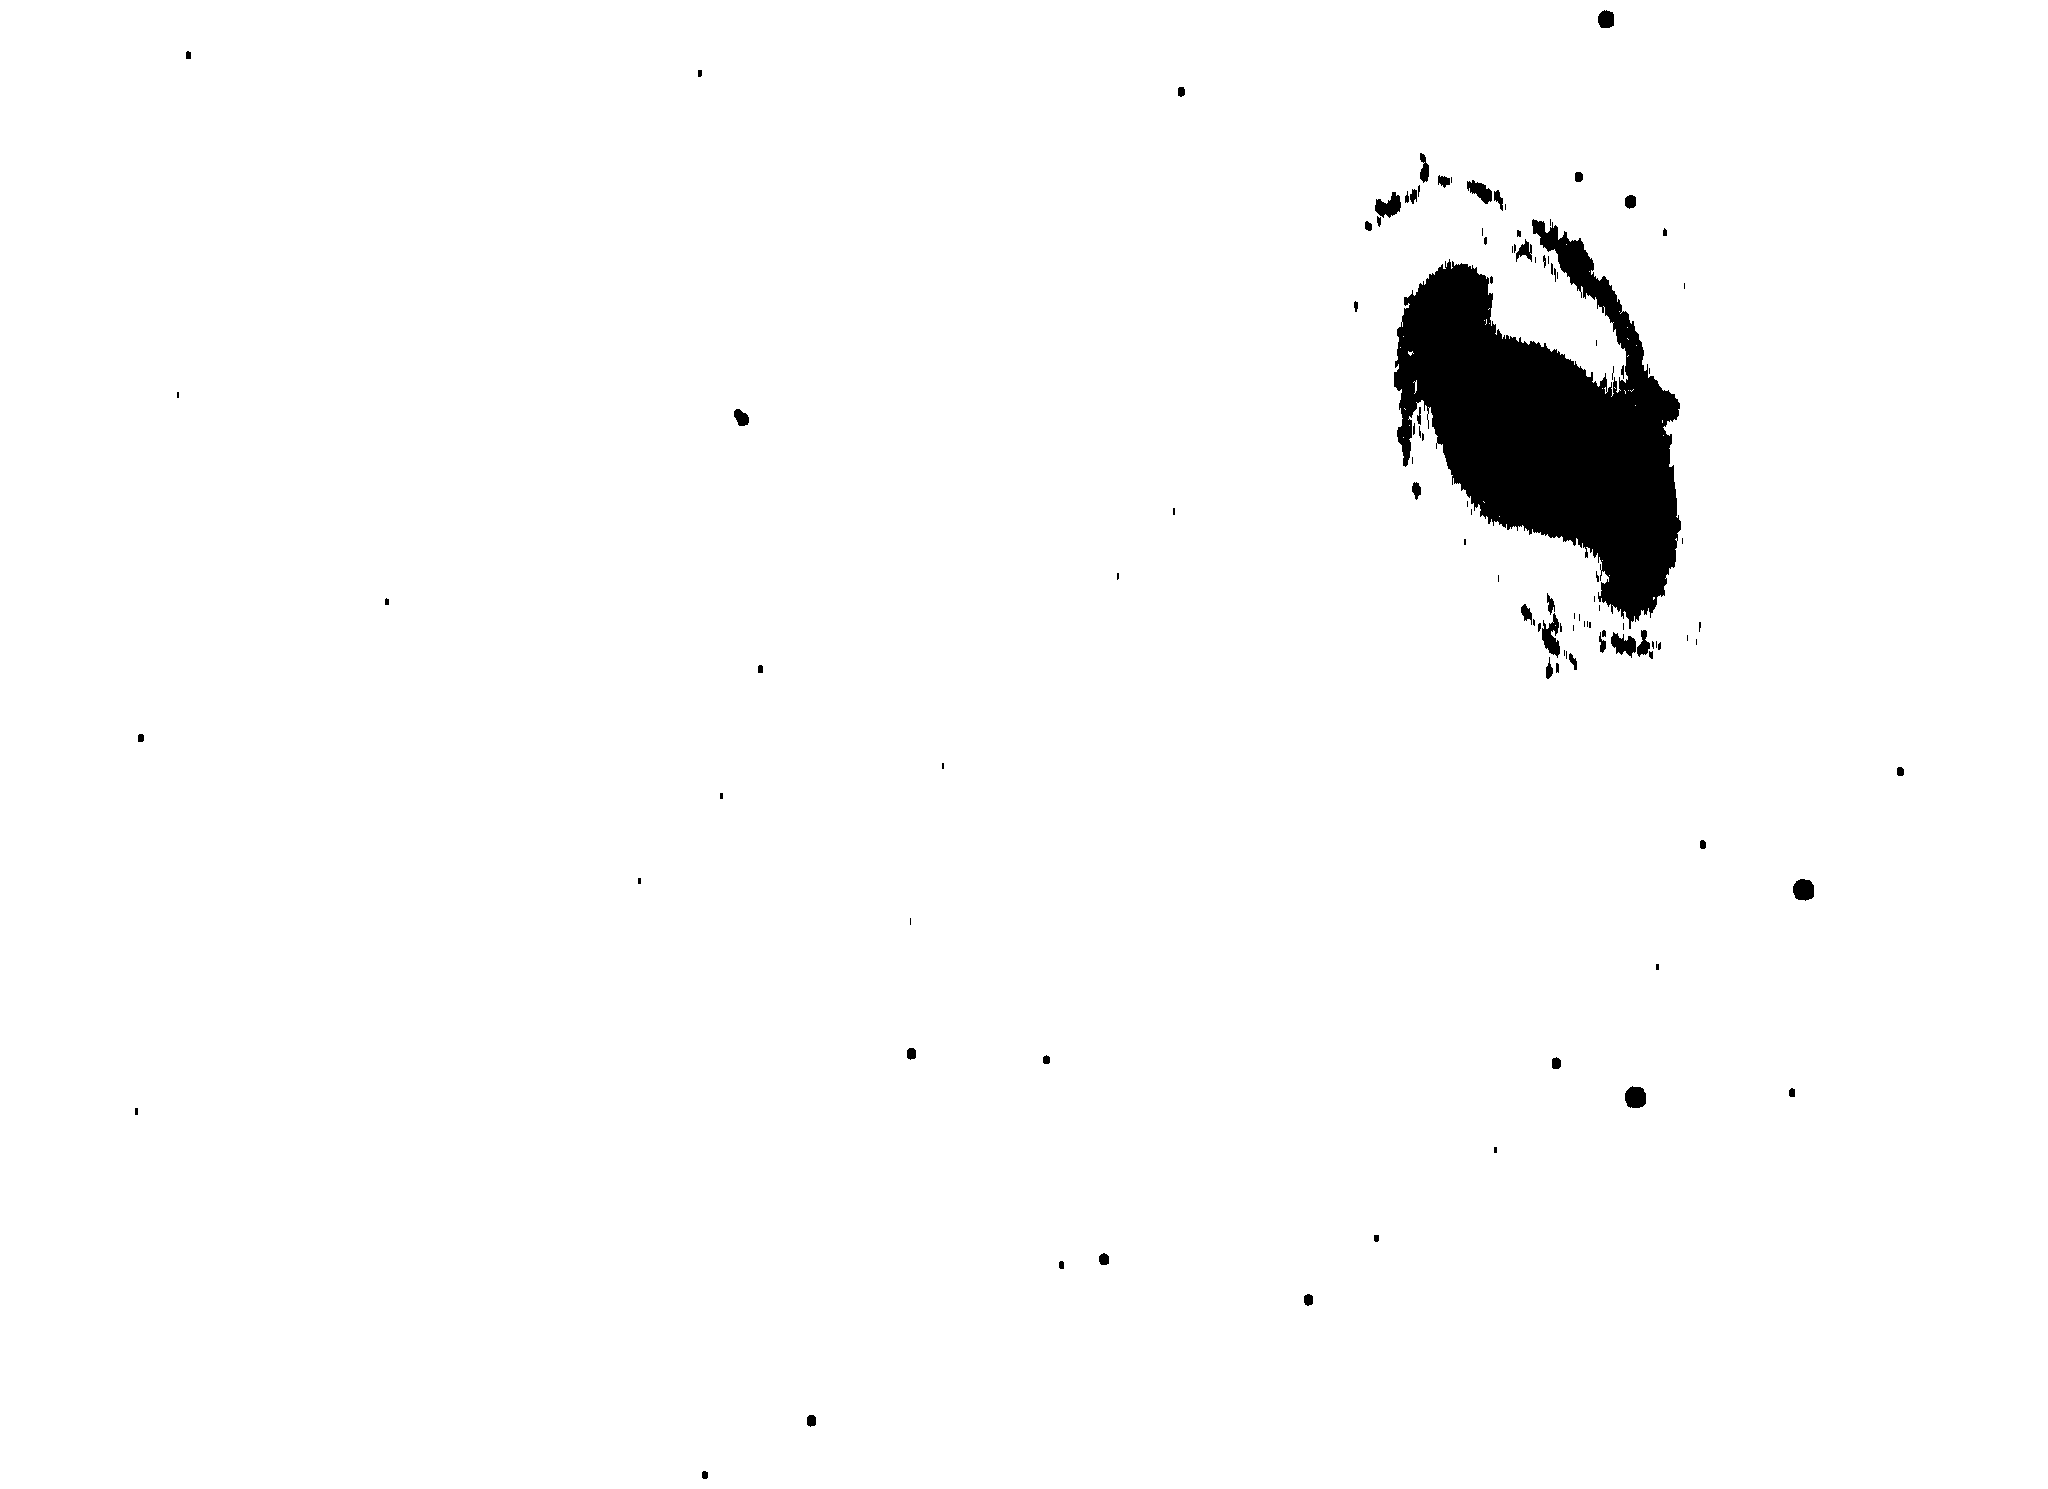
\includegraphics[width=8cm]{img4.png}}
\caption{Operación cierre.}
\label{fig:img4}
\end{figure}

Una vez que se tiene una imagen binaria y con solo los elementos más brillantes de la imagen original, creé un detector de \textit{blobs}, como se explica en la siguiente sección.

\subsection{Blob detection}

Un \textit{blob} es un grupo de píxeles de una imagen que comparten la propiedad de tener valores similares. En la figura \ref{fig:img4} cada región oscura aislada es un \textit{blob}, y el objetivo de esta sección es detectarlos.

En OpenCV se dispone de la función \textbf{SimpleBlobDetector} para lograr esto. Basta con fijar una serie de parámetros que se refieren a unas características básicas (a saber: color, tamaño y forma).

El siguiente código muestra el detector de \textit{blobs} que creé y los parámetros con los que obtuve mejores resultados, que son una convexidad mínima de 0.5 y un valor de la elongación mínimo de 0.1:

\lstinputlisting[language=Python, frame= single, firstline=21]{blobDetection.py}
y la figura \ref{fig:img5} muestra el resultado de aplicar el detector de \textit{blobs}.
\begin{figure}[h!]
\centering
\fbox{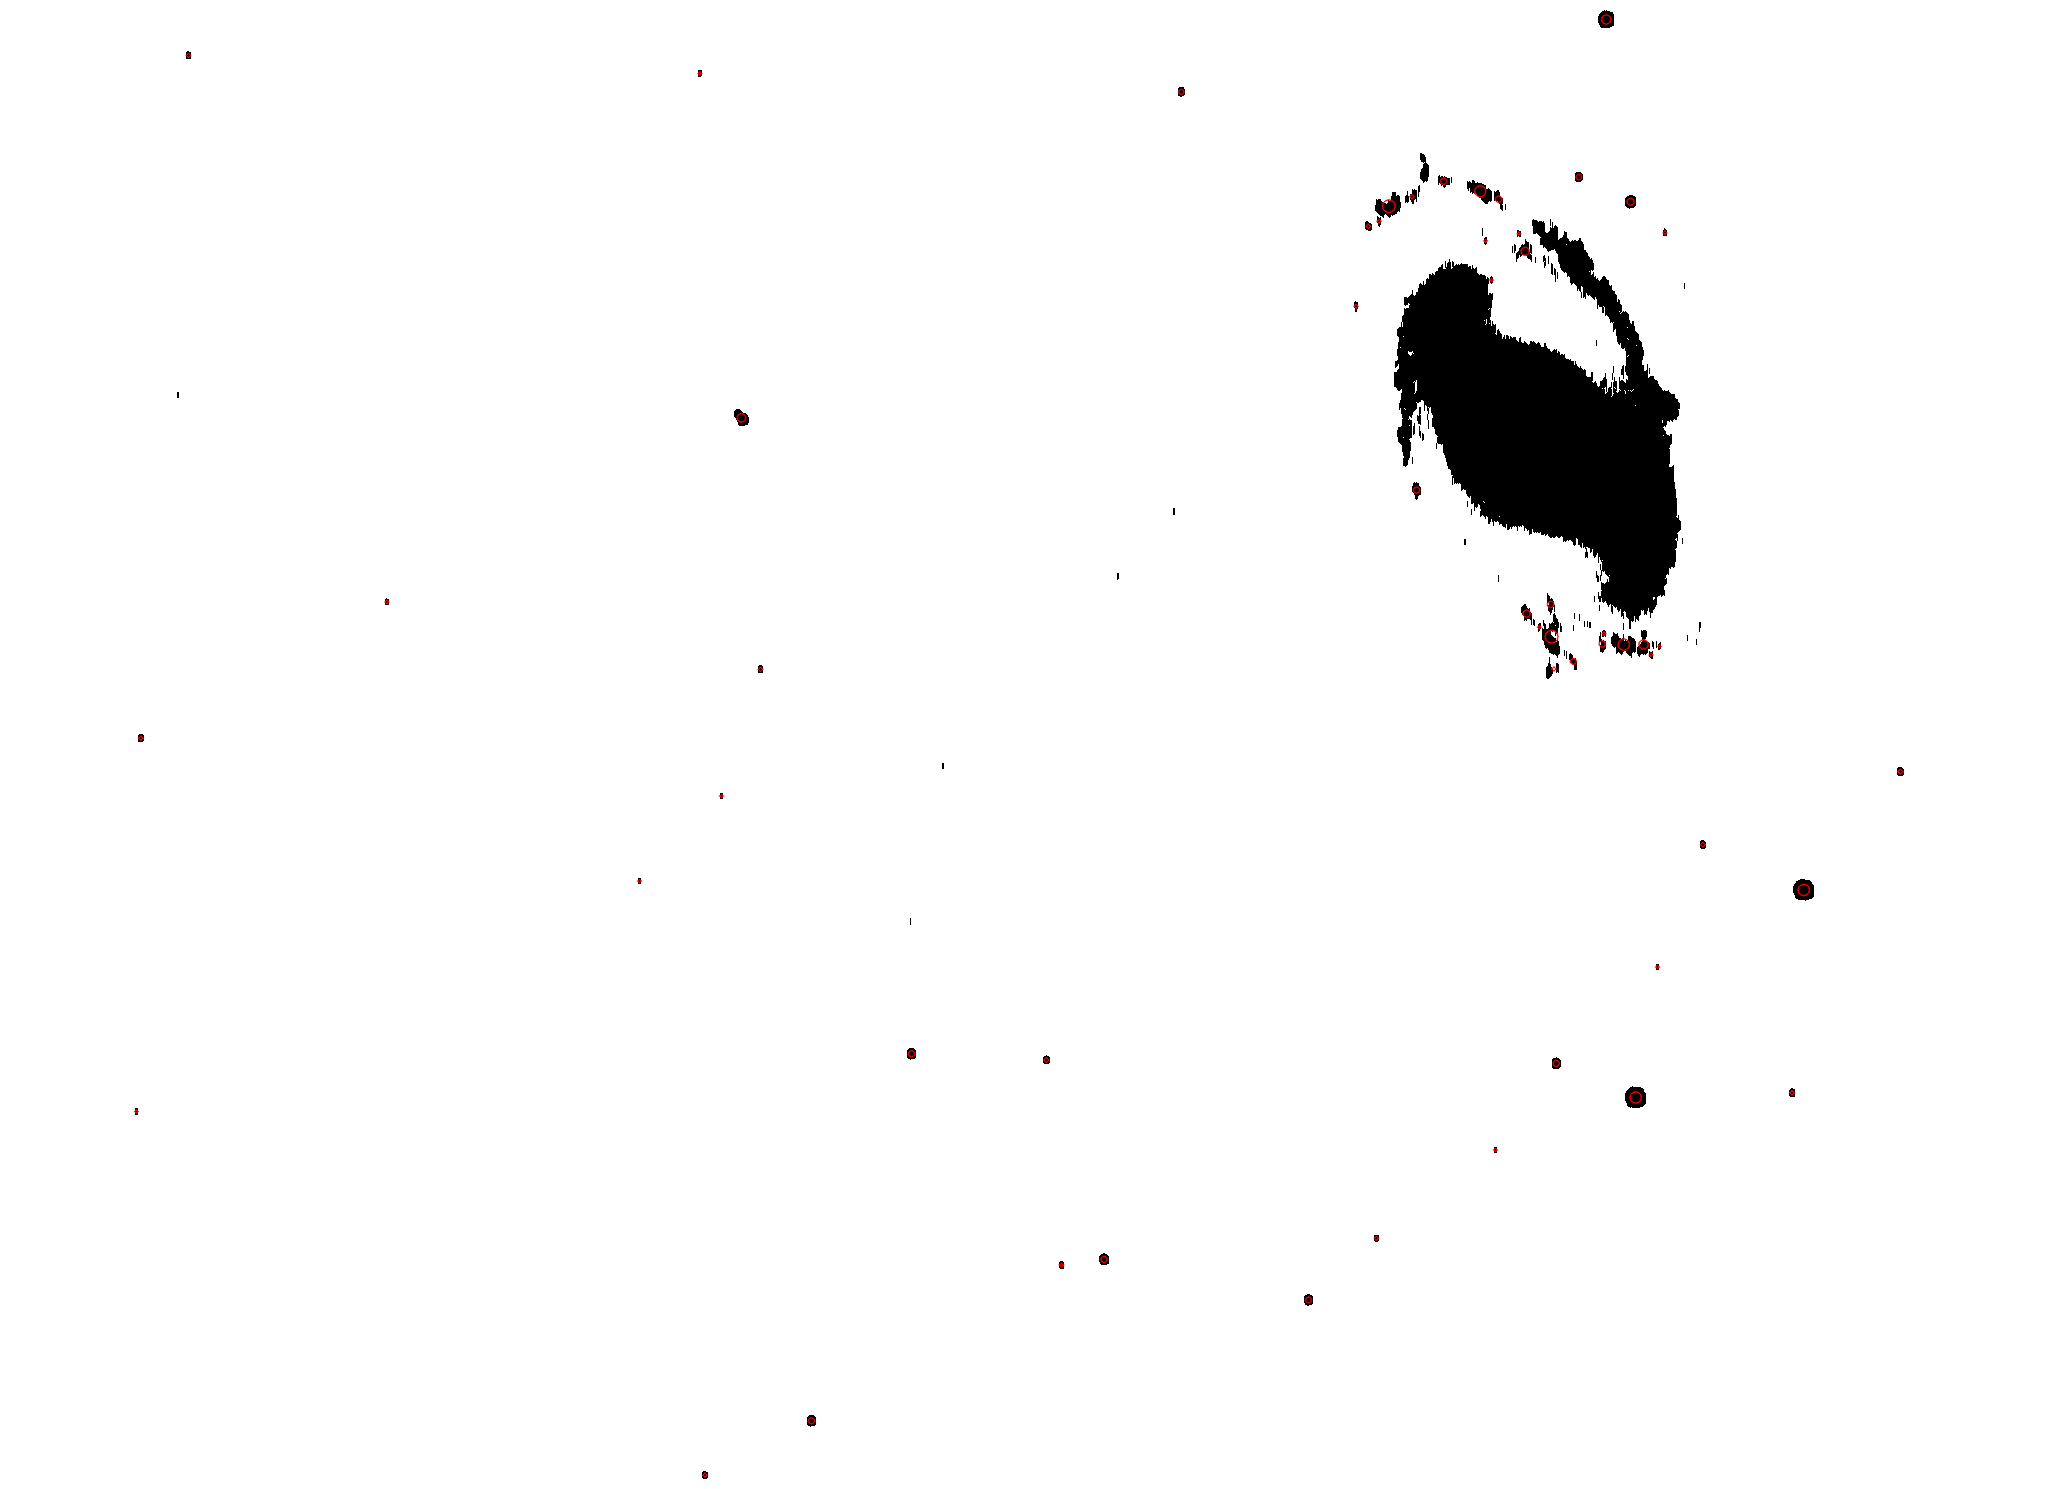
\includegraphics[width=8cm]{img5.png}}
\caption{Detección de \textit{blobs}.}
\label{fig:img5}
\end{figure}

En la figura \ref{fig:img6} se ve en detalle una región de la imagen \ref{fig:img5}.
\begin{figure}[h!]
\centering
\fbox{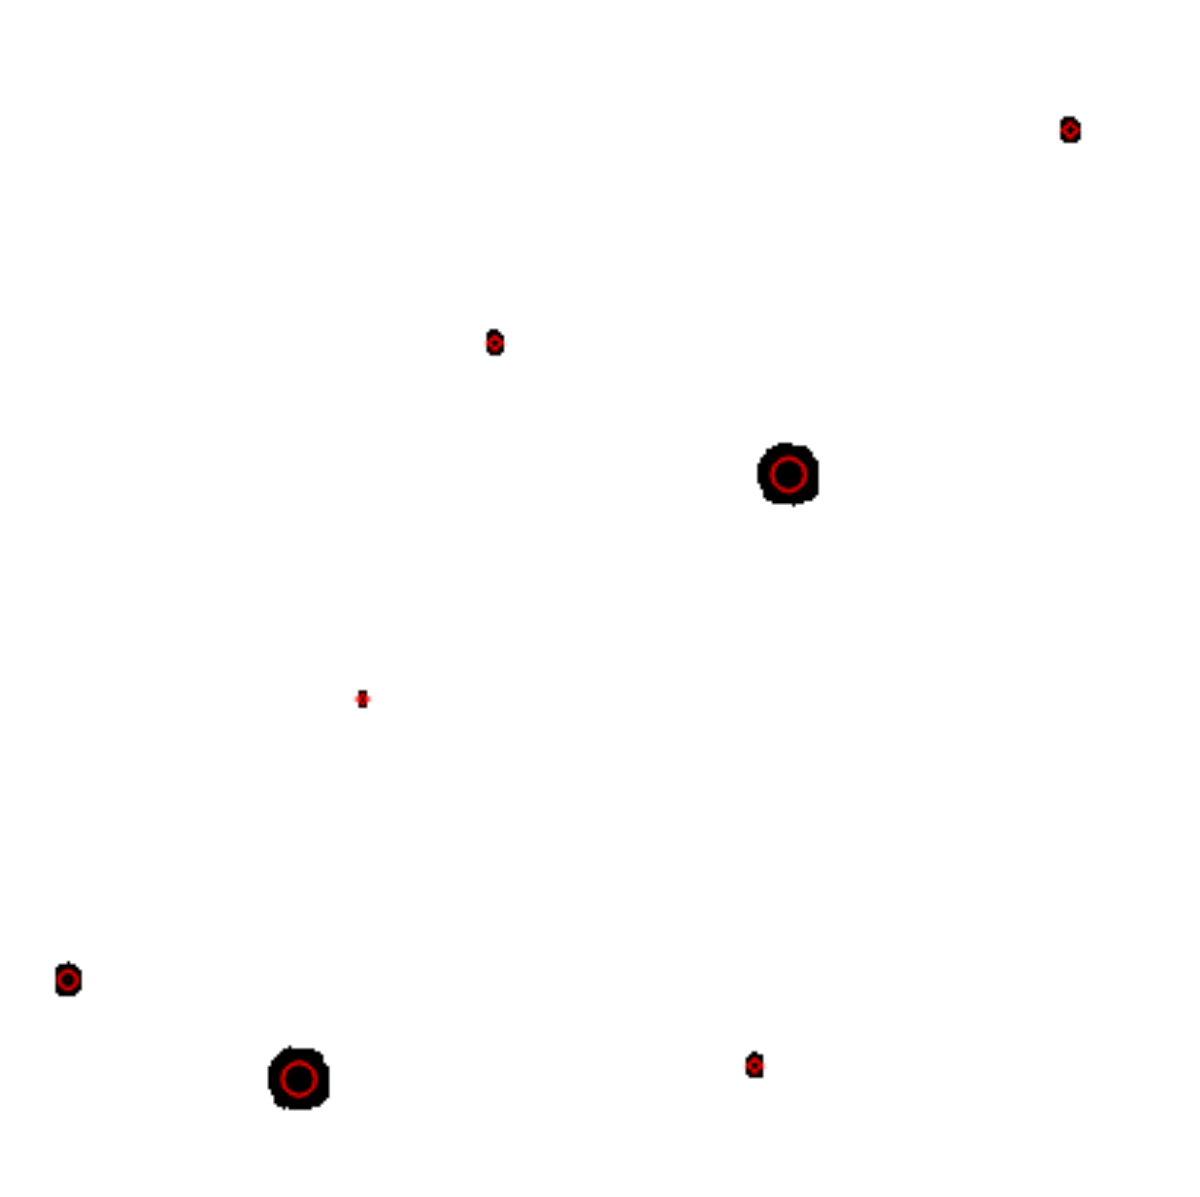
\includegraphics[width=5cm]{img5Zoom.png}}
\caption{Detección de \textit{blobs} en detalle.}
\label{fig:img6}
\end{figure}

\section{Conclusión y trabajo futuro}
En resumen, se han definido métodos para, partiendo de una imagen de un fichero FITS, identificar tanto las grandes regiones luminosas candidatas a galaxias como objetos más brillantes de la imagen. El siguiente paso sería continuar con la clasificación de las imágenes ya simplificadas y separadas en sus zonas de interés. Esto se podría hacer de varias maneras. Por ejemplo, si se dispusiera de una gran base de datos con ficheros FITS etiquetados por los objetos astronómicos que contienen, se podrían usar técnicas de Machine Learning para crear clasificadores automáticos con ajuste dinámico de los parámetros de todas las funciones usadas.



\section{Problemas encontrados}
A la hora de realizar este trabajo me he encontrado principalmente con dos problemas. El primero es la falta de imágenes con las que trabajar y sobre todo de calidad adecuada para trabajar con ellas a nivel amateur-académico iniciado. Si bien se pueden encontrar muchos sitios web con ficheros FITS de acceso libre tras buscar un poco en Internet, pocos eran los que disponían de una base de datos que alguien profano en la materia pudiera entender y manejar con soltura en un primer acercamiento al manejo de los mismos.

Finalmente di con el sitio web de un proyecto que libera ficheros FITS etiquetados por su contenido, lo que me resultó muy útil para acceder de manera directa a imágenes de galaxias, a fin de empezar a trabajar con ellas. Este sitio es "The Sloan Digital Sky Survey: Mapping the Universe" (www.sdss.org). Lamentablemente para mí, el buscador interno de la página dejó de funcionar y tuve problemas para conseguir nuevos ficheros con los que trabajar.

El segundo problema es la naturaleza de las imágenes captadas por los telescopios. Al ser el principal objetivo del trabajo aprender a usar OpenCV, intenté primero obtener resultados haciendo uso de sus funciones predefinidas, pero me encontré con que parecían estar hechas principalmente para su aplicación en imágenes tomadas en el espectro visible. Las imágenes astrónomicas obtenidas de los ficheros FITS distan mucho de ser tan nítidas como las obtenidas por cualquier cámara de fotos, y si se representan tal y como son leídas directamente del FITS probablemente no se distingan nada más que gránulos grises. Esto es de esperar, puesto que no están hechas para ser mostradas, al menos, en crudo, pero explica por qué necesité crear mi propio filtro para obtener algún resultado. Una vez superado esto pude satisfactoriamente hacer uso de las funciones de OpenCV.


\label{sec:Problemas}


\appendix
\section{Apéndices}
\subsection{Muestras del procesado de otras imágenes}
\subsection{Trabajo descartado}
\subsubsection{Morphology}
\label{sec:morf}
testMorefilters
\subsubsection{Canny}
testCanny
\subsubsection{Sobel}
testEdges
\subsubsection{Flow}
testFlow
\subsubsection{3d}
test3d
\section{Bibliografía}


%\listoffigures
%\listoftables

\clearpage
\end{document}
